\input templates/header


\title[ASD - Strutture speciali]{\textbf{Algoritmi e Strutture Dati}\\[24pt]
Strutture dati speciali}

\graphicspath{{figs/10/}}

\usepackage[export]{adjustbox}
\begin{document}



%-------------------------------------------------------------------------
\FrameTitle{}

%-------------------------------------------------------------------------
\FrameContent

%%%%%%%%%%%%%%%%%%%%%%%%%%%%%%%%%%%%%%%%%%%%%%%%%%%%%%%%%%%%%%%%%%%%%%%%%%
\section{Introduzione}
%%%%%%%%%%%%%%%%%%%%%%%%%%%%%%%%%%%%%%%%%%%%%%%%%%%%%%%%%%%%%%%%%%%%%%%%%%

%-------------------------------------------------------------------------
\begin{frame}{Introduzione}

\BB{Strutture dati viste finora}
\BIL
\item Sequenze, insiemi e dizionari
\EIL

\BB{Strutture “speciali”}
\BIL
\item Se non tutte le operazioni sono necessarie, è possibile realizzare strutture dati più efficienti, “specializzate” per particolare compiti
\item Le operazioni base (inserimento, cancellazione, lettura, etc.) possono non essere sufficienti: a volte servono operazioni speciali
\EIL

\end{frame}

%-------------------------------------------------------------------------
\begin{frame}{Esempi}

\BIL
\item \alert{Code con priorità}
\item \alert{Insiemi disgiunti}
\item Interval/segment tree
\item K-D tree
\item Trie
\item Fenvick Tree
\item Merkle tree
\item Secondo Wikipedia, 338 pagine nella categoria strutture dati...
\EIL
    
\end{frame}


%%%%%%%%%%%%%%%%%%%%%%%%%%%%%%%%%%%%%%%%%%%%%%%%%%%%%%%%%%%%%%%%%%%%%%%%%%
\section{Code con priorità}
\subsection{Introduzione}
%%%%%%%%%%%%%%%%%%%%%%%%%%%%%%%%%%%%%%%%%%%%%%%%%%%%%%%%%%%%%%%%%%%%%%%%%%

\begin{frame}{Code con priorità}

\vspace{-9pt}
\begin{myboxtitle}[Definizione (\alert{Priority Queue})]
Una \alert{coda con priorità} è una struttura dati astratta, simile ad 
una coda, in cui ogni elemento inserito possiede una sua "\alert{priorità}"
\small
\BIL
\item \alert{Min-priority queue}: estrazione per valori crescenti di priorità
\item \alert{Max-priority queue}: estrazione per valori decrescenti di priorità
\EIL
\end{myboxtitle}

\begin{myboxtitle}[Operazioni permesse]
\BIL
\item Inserimento in coda
\item Estrazione dell'elemento con priorità di valore min/max
\item Modifica priorità (decremento/incremento) di un elemento inserito
\EIL
\end{myboxtitle}

\end{frame}

%---------------------------------------------------------------------------
\begin{frame}[shrink=8]{Specifica}

\vspace{-12pt}
\begin{Procedure}
\caption[A]{\textsc{MinPriorityQueue}}

\BlankLine
\textcolor{blue}{\% Crea una coda con priorità con capacità $n$, vuota}\;
\Heap \heapconstructor(\INTEGER\ $n$)\;

\BlankLine
\textcolor{blue}{\% Restituisce \TRUE\ se la coda con priorità è vuota}\;
\BOOLEAN \setempty()\; 

\BlankLine
\textcolor{blue}{\% Restituisce l'elemento minimo di una coda con priorità non vuota}\;
\Item \heapmin()\;

\BlankLine
\textcolor{blue}{\% Rimuove e restituisce il minimo da una coda con priorità non vuota}\;
\Item \heapdeletemin()\;
 
\BlankLine
\textcolor{blue}{\% Inserisce l'elemento $x$ con priorità $p$ nella coda con priorità. Restituisce}\;
\textcolor{blue}{\% un oggetto \PriorityItem che identifica $x$ all'interno della coda}\;
\PriorityItem \heapinsert(\Item\ $x$, \INTEGER $p$)\;

\BlankLine
\textcolor{blue}{\% Diminuisce la priorità dell'oggetto identificato da $y$ portandola a $p$}\;
\heapdecrease(\PriorityItem $y$, \INTEGER $p$)\;

\BlankLine
\end{Procedure}

\end{frame}

\begin{frame}{Reality Check -- Simulatore event-driven}

\vspace{-9pt}
\BIL
\item Ad ogni evento è associato un timestamp di esecuzione
\item Ogni evento può generare nuovi eventi, con timestamp arbitrari
\item Una coda con min-priorità può essere utilizzata per eseguire gli eventi in ordine di timestamp
\EIL

\medskip
\IG{0.95}{events.pdf}



\end{frame}

\begin{frame}{Applicazioni nelle prossime lezioni}
\BIL
\item Algoritmo di Dijkstra
\item Codifica di Huffmann
\item Algoritmo di Prim per gli alberi di copertura di peso minimo
\EIL
\end{frame}



\begin{frame}{Implementazioni}

\begin{center}
\begin{tabular}{|c|c|c|c|c|}
\hline
Metodo & Lista/vettore  & Lista & Vettore & Albero \\
       & non ordinato  & Ordinata & Ordinato & RB \\\hline
\heapmin()         & $O(n)$ & $O(1)$ & $O(1)$      & $O(\log n)$ \\\hline
\heapdeletemin()   & $O(n)$ & $O(1)$ & $O(n)$      & $O(\log n)$ \\\hline
\heapinsert()      & $O(n)$ & $O(n)$ & $O(n)$      & $O(\log n)$ \\\hline
\heapdecrease()    & $O(n)$ & $O(n)$ & $O(\log n)$ & $O(\log n)$ \\\hline
\end{tabular} 
\end{center}

\begin{myboxtitle}[Heap]
Una struttura dati speciale che associa 
\BI
\item i vantaggi di un albero (esecuzione in tempo $O(\log n)$), e 
\item i vantaggi di un vettore (memorizzazione efficiente)
\EI
\end{myboxtitle}

\end{frame}

\begin{frame}{Heap}
    
\vspace{-9pt}
\begin{myboxtitle}[Storia]
\BIL
\item Struttura dati inventata da J. Williams nel 1964
\item Utilizzata per implementare un nuovo algoritmo di ordinamento: \alert{HeapSort}
\item Williams intuì subito che poteva essere usata per altri scopi
\item Seguiamo l'approccio storico nel presentare gli heap
  \BI
  \item Prima HeapSort
  \item Poi Code con priorità
  \EI
\EIL
\end{myboxtitle}

\end{frame}


\subsection{Vettore heap}

\begin{frame}{Alberi binari}

\vspace{-9pt}
\begin{myboxtitle}[Albero binario perfetto]
\BIL
\item Tutte le foglie hanno la stessa profondità $h$
\item Nodi interni hanno tutti grado $2$
\item Dato il numero di nodi $n$, ha altezza $h = \lfloor \log n \rfloor$
\item Dato l'altezza $h$, ha numeri di nodi $n=2^{h+1}-1$
\EIL
\end{myboxtitle}

\centering
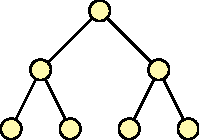
\includegraphics[width=4cm]{perfetto.pdf}

\end{frame}

\begin{frame}{Alberi binari}

\vspace{-9pt}
\begin{myboxtitle}[Albero binario completo]
\BIL
\item Tutte le foglie hanno profondità $h$ o $h-1$
\item Tutti i nodi a livello $h$ sono “accatastati” a sinistra
\item Tutti i nodi interni hanno grado 2, eccetto al più uno
\item Dato il numero di nodi $n$, ha altezza $h = \lfloor \log n \rfloor$
\EIL
\end{myboxtitle}

\centering
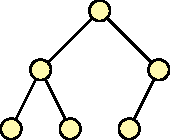
\includegraphics[width=4cm]{completo.pdf}

\end{frame}

\begin{frame}{Alberi binari heap}

\vspace{-9pt}
\begin{myboxtitle}[Proprietà heap]
Un \alert{albero max-heap} (\alert{min-heap}) è un albero binario 
completo tale che il valore memorizzato in ogni nodo è \alert{maggiore} (\alert{minore}) dei valori memorizzati nei suoi figli.
\end{myboxtitle}

\vspace{-6pt}
\begin{columns}[T]
\column{0.52\textwidth}

\begin{myboxtitle}[Note]
Le definizioni e gli algoritmi per alberi max-heap sono simmetrici rispetto
agli algoritmi per alberi min-heap
\end{myboxtitle}

\column{0.44\textwidth}
\vspace{-6pt}
\IG{0.8}{esempio1.pdf}
\end{columns}

\end{frame}

\begin{frame}{Alberi binari heap}

\BIL
\item Un albero heap non impone una relazione di \alert{ordinamento totale} fra i figli di un nodo
\item Un albero heap è un \alert{ordinamento parziale}
  \BI
  \item \alert{Riflessivo}: Ogni nodo è $\geq$ di se stesso
  \item \alert{Antisimmetrico}: se $n \geq m$ e $m \geq n$, allora $m=n$
  \item \alert{Transitivo}: se $n \geq m$ e $m \geq r$, allora $n \geq r$
  \EI
\item Ordinamenti parziali
  \BI
  \item Nozione più debole di un ordinamento totale...
  \item ... ma più semplice da costruire
  \EI
\EIL

\end{frame}

\begin{frame}{Alberi binari heap}

\vspace{-12pt}
\small
\begin{columns}[T]
\column{0.55\textwidth}
\begin{myboxtitle}[Vettore heap]
Un albero heap può essere rappresentato tramite un \alert{vettore heap} 
\end{myboxtitle}

\begin{myboxtitle}[Memorizzazione ($A \lbrack 1 \ldots n \rbrack$)]
  \renewcommand*{\arraystretch}{1.2}
  \begin{tabular}{ll}
    \alert{Radice} & $root() = 1$\\
    \alert{Padre nodo $i$} & $p(i) = \lfloor i/2 \rfloor$\\
    \alert{Figlio sx nodo $i$} & $l(i) = 2i$\\
    \alert{Figlio dx nodo $i$} & $r(i) = 2i+1$\\
  \end{tabular}
\end{myboxtitle}

\column{0.40\textwidth}
\vspace{-12pt}
\IG{1.0}{esempio-vettore1.pdf}
\end{columns}


\IG{0.7}{vettore1.pdf}

\end{frame}

\begin{frame}{Alberi binari heap}

\vspace{-12pt}
\small
\begin{columns}[T]
\column{0.55\textwidth}
\begin{myboxtitle}[Vettore heap]
Un albero heap può essere rappresentato tramite un \alert{vettore heap} 
\end{myboxtitle}

\begin{myboxtitle}[Memorizzazione ($A \lbrack 0 \ldots n-1 \rbrack$)]
  \renewcommand*{\arraystretch}{1.2}
  \begin{tabular}{ll}
    \alert{Radice} & $root() = 0$\\
    \alert{Padre nodo $i$} & $p(i) = \lfloor (i-1)/2 \rfloor$\\
    \alert{Figlio sx nodo $i$} & $l(i) = 2i+1$\\
    \alert{Figlio dx nodo $i$} & $r(i) = 2i+2$\\
  \end{tabular}
\end{myboxtitle}
\column{0.40\textwidth}
\vspace{-12pt}
\IG{1.0}{esempio-vettore0.pdf}
\end{columns}

\IG{0.7}{vettore0.pdf}

\end{frame}

\begin{frame}{Alberi binari heap}

\vspace{-9pt}
\begin{myboxtitle}[Proprietà max-heap su vettore]
\[
A[i] \geq A[l(i)], A[i] \geq A[r(i)]
\]
\end{myboxtitle}

\begin{myboxtitle}[Proprietà min-heap su vettore]
\[
A[i] \leq A[l(i)], A[i] \leq A[r(i)]
\]
\end{myboxtitle}


\end{frame}

\subsection{HeapSort}

\begin{frame}{HeapSort}

\vspace{-9pt}
\begin{myboxtitle}[Organizzazione \heapsort()]
Ordina un max-heap "in-place", prima costruendo un max-heap nel vettore e poi spostando l'elemento max in ultima posizione, ripristinando la proprietà max-heap
\BIL
\item \alert{\heapbuild()}\\ Costruisce un max-heap a partire da un vettore non ordinato 
\item \alert{\maxheapify()}\\ Ripristina la proprietà max-heap
\EIL
\end{myboxtitle}


\end{frame}

\begin{frame}{maxHeapRestore()}

\vspace{-9pt}
\begin{myboxtitle}[Input]
Un vettore $A$ e un indice $i$, tale per cui gli alberi binari
con radici\\ $l(i)$ e $r(i)$ sono max-heap
\end{myboxtitle}

\begin{myboxtitle}[Osservazione]
\BI
\item \EE possibile che $A[i]$ sia minore di $A[l(i)]$ o $A[r(i)]$
\item In altre parole, non è detto che il sottoalbero con radice $i$\\ sia
un max-heap
\EI
\end{myboxtitle}

\begin{myboxtitle}[Goal]
Modificare in-place il vettore $A$ in modo tale che l'albero binario\\ con radice $i$
sia un max-heap
\end{myboxtitle}    
    
\end{frame}

\begin{frame}{Esempio}

\centering
\begin{overprint}[0.5\textwidth]
\onslide<1|handout:1>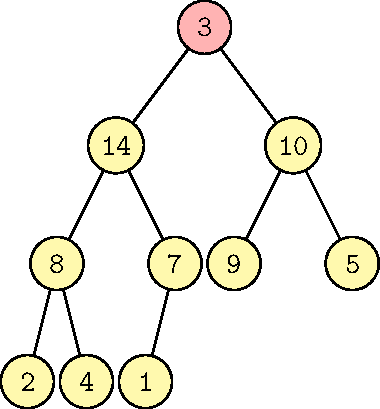
\includegraphics[width=1.0\textwidth,page=1]{esempio-errato.pdf}
\onslide<2|handout:0>\includegraphics[width=1.0\textwidth,page=2]{esempio-errato.pdf}
\onslide<3|handout:2>\includegraphics[width=1.0\textwidth,page=3]{esempio-errato.pdf}
\onslide<4|handout:0>\includegraphics[width=1.0\textwidth,page=4]{esempio-errato.pdf}
\onslide<5|handout:3>\includegraphics[width=1.0\textwidth,page=5]{esempio-errato.pdf}
\onslide<6|handout:0>\includegraphics[width=1.0\textwidth,page=6]{esempio-errato.pdf}
\onslide<7|handout:4>\includegraphics[width=1.0\textwidth,page=7]{esempio-errato.pdf}
\end{overprint}

\end{frame}    

\begin{frame}{Ripristinare la proprietà max-heap}

\vspace{-9pt}
\begin{Procedure}
\caption[A]{\maxheapify($\Item[\,]\ A$, \INTEGER $i$, \INTEGER \heapcount)}

\INTEGER $\Max = i$\;
\If{$\heapleft(i) \leq \heapcount$ \AND $A[\heapleft(i)] > A[\Max]$}
{
  $\Max = \heapleft(i)$
}
\If{$\heapright(i) \leq \heapcount$ \AND $A[\heapright(i)] > A[\Max]$}
{
  $\Max = \heapright(i)$
}
\If{$i \neq \Max$}
{
  $\Swap(A,i,\Max)$\;
  $\maxheapify(A, \Max, \heapcount)$\;
}
\end{Procedure}

\BB{Qual è la complessità computazionale di $\maxheapify()$?}


\end{frame}

\begin{frame}{\textsf{maxHeapRestore}() -- Complessità computazionale}

\vspace{-9pt}
\BB{Qual è la complessità computazionale di $\maxheapify()$?}

\BI
\item Ad ogni chiamata, vengono eseguiti $O(1)$ confronti
\item Se il nodo $i$ non è massimo, si richiama ricorsivamente
\maxheapify() su uno dei figli 
\item L'esecuzione termina quando si raggiunge una foglia
\item L'altezza dell'albero è pari a $\lfloor \log n \rfloor$
\EI

\bigskip
\BB{Complessità}
\[
  T(n) = O(\log n)
\]

\end{frame}

\begin{frame}{Dimostrazione correttezza (per induzione sull'altezza)}

\vspace{-9pt}
\begin{myboxtitle}[Teorema]
Al termine dell'esecuzione, l'albero radicato in $A[i]$
rispetta la proprietà max-heap
\end{myboxtitle}

\pause
\begin{myboxtitle}[Caso base: altezza $h=0$]
Se $h=0$, l'albero è dato da un solo nodo che rispetta la
proprietà heap
\end{myboxtitle}

\begin{myboxtitle}[Ipotesi induttiva]
L'algoritmo funziona correttamente su tutti gli alberi di altezza minore di $h$
\end{myboxtitle}

\end{frame}

\begin{frame}{Dimostrazione correttezza (per induzione sull'altezza)}

\vspace{-12pt}
\begin{columns}[T]
\column{0.50\textwidth}
\BB{Induzione - Altezza $h$ - Caso 1}

\medskip
$A[i] \geq A[l(i)], A[i] \geq A[r(i)]$:
  \BI
  \item L'albero radicato in $A[i]$ rispetta la proprietà max-heap 
  \item L'algoritmo termina (CVD)
  \EI
\column{0.45\textwidth}

\vspace{-6pt}
\IG{1.0}{dimostrazione.pdf}
\end{columns}
\end{frame}

\begin{frame}{Dimostrazione correttezza (per induzione sull'altezza)}

\small
\vspace{-9pt}
\begin{columns}[T]
\column{0.50\textwidth}
\BB{Induzione - Altezza $h$ - Caso 2}

\medskip
\alert<1|handout:1>{$A[l(i)] > A[i], A[l(i)] > A[r(i)]$}:
  \BI
  \item \alert<2|handout:2>{Viene fatto uno scambio $A[i] \leftrightarrow A[l(i)]$}
  \item \alert<3|handout:3>{Dopo lo scambio, $A[i] \geq A[l(i)], A[i] \geq A[r(i)]$}
  \item \alert<4|handout:4>{Il sottoalbero $A[r(i)]$ è inalterato e rispetta la proprietà heap}
  \item \alert<5|handout:5>{Il sottoalbero $A[l(i)]$ può aver perso la proprietà heap}
  \item \alert<6|handout:6>{Si applica $\maxheapify()$ ricorsivamente su di $A[l(i)]$, che ha altezza minore di $h$}
  \EI
\column{0.45\textwidth}

\begin{overprint}
\includegraphics<1|handout:1>[width=1.0\textwidth,page=2]{dimostrazione.pdf}
\includegraphics<2|handout:2>[width=1.0\textwidth,page=3]{dimostrazione.pdf}
\includegraphics<3|handout:3>[width=1.0\textwidth,page=4]{dimostrazione.pdf}
\includegraphics<4|handout:4>[width=1.0\textwidth,page=5]{dimostrazione.pdf}
\includegraphics<5|handout:5>[width=1.0\textwidth,page=6]{dimostrazione.pdf}
\includegraphics<6|handout:6>[width=1.0\textwidth,page=7]{dimostrazione.pdf}
\includegraphics<7|handout:7>[width=1.0\textwidth,page=8]{dimostrazione.pdf}
\end{overprint}

\BB{Passo induttivo - Caso 3}

\medskip
Simmetrico rispetto al Caso 2

\end{columns}
\end{frame}

\begin{frame}{heapBuild()}

\vspace{-9pt}
\begin{myboxtitle}[Principio di funzionamento]
\TwoColsCustom{0.8}{0.20}{
\smallskip
\BIL
\item Sia $A[1 \ldots n]$ un vettore da ordinare
\item Tutti i nodi $A[\lfloor n/2 \rfloor+1 \ldots n]$ sono foglie dell'albero e quindi heap contenenti \alert{1} elemento
\item La procedura \heapbuild() 
  \BI
  \item attraversa i restanti nodi dell'albero, a partire da $\lfloor n/2 \rfloor$ fino ad $1$
  \item esegue \maxheapify() su ognuno di essi
  \EI
\EIL
}{
}
\end{myboxtitle}
\begin{Procedure}
\caption[A]{\heapbuild($\Item[\,]\ A$, \INTEGER $n$)}
\label{alg:heapbuild}

\For{$i = \lfloor n/2 \rfloor$ \DOWNTO $1$}
{
  $\maxheapify(A, i, n)$\;
}
\end{Procedure}

\end{frame}

\begin{frame}{Esempio}

\small
\begin{columns}[T]
\column{0.45\textwidth}
\BIL
\item I nodi $A[\lfloor n/2 \rfloor+1 \ldots n]$ sono foglie dell'albero 
e quindi heap di un elemento 
\item Per ogni posizione da $\lfloor n/2 \rfloor$ fino ad $1$, si esegue \maxheapify()
\EIL
\column{0.45\textwidth}
\vspace{-12pt}
\begin{overprint}
\onslide<1|handout:1>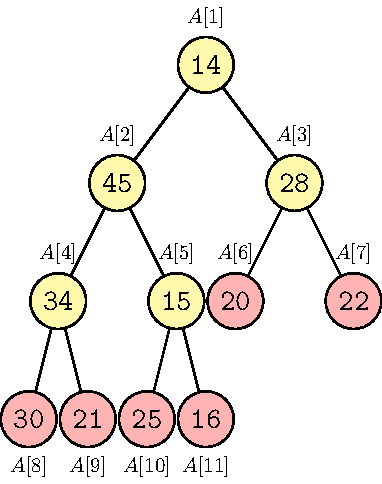
\includegraphics[width=\textwidth,page=1]{heapbuild.pdf}
\onslide<2|handout:0>\includegraphics[width=\textwidth,page=2]{heapbuild.pdf}
\onslide<3|handout:0>\includegraphics[width=\textwidth,page=3]{heapbuild.pdf}
\onslide<4|handout:0>\includegraphics[width=\textwidth,page=4]{heapbuild.pdf}
\onslide<5|handout:0>\includegraphics[width=\textwidth,page=5]{heapbuild.pdf}
\onslide<6|handout:0>\includegraphics[width=\textwidth,page=6]{heapbuild.pdf}
\onslide<7|handout:0>\includegraphics[width=\textwidth,page=7]{heapbuild.pdf}
\onslide<8|handout:0>\includegraphics[width=\textwidth,page=8]{heapbuild.pdf}
\onslide<9|handout:0>\includegraphics[width=\textwidth,page=9]{heapbuild.pdf}
\onslide<10|handout:2>\includegraphics[width=\textwidth,page=10]{heapbuild.pdf}
\end{overprint}
\end{columns}

\end{frame}

\begin{frame}{Correttezza}

\vspace{-9pt}
% \begin{overprint}
% \onslide<1|handout:0>
% \BB{Invariante di ciclo?}
%
% \onslide<2|handout:1>
\begin{myboxtitle}[Invariante di ciclo]
All'inizio di ogni iterazione del ciclo \FOR, i nodi $[i+1, \ldots, n]$ sono radice di uno heap.
\end{myboxtitle}


\begin{myboxtitle}[Dimostrazione -- Inizializzazione]
\BIL
\item All'inizio, $i= \lfloor n/2 \rfloor$. 
\item Supponiamo che $\lfloor n/2 \rfloor+1$ non sia una foglia
\item Quindi ha almeno il figlio sinistro: $2\lfloor n/2 \rfloor+2$
\item Questo ha indice $n+1$ oppure $n+2$, assurdo perché $n$ è la dimensione
massima
\item La dimostrazione vale per tutti gli indici successivi
\EIL 
\end{myboxtitle}

% \end{overprint}


\end{frame}

\begin{frame}{Correttezza}

\vspace{-12pt}
\begin{overprint}
\onslide<1|handout:1>
\begin{myboxtitle}[Invariante di ciclo]
All'inizio di ogni iterazione del ciclo \FOR, i nodi $[i+1, \ldots, n]$ sono radice di uno heap.
\end{myboxtitle}

\begin{myboxtitle}[Dimostrazione -- Conservazione]
\BIL
\item \EE possibile applicare $\maxheapify$ al nodo $i$, perché
$2i < 2i+1 \leq n$ sono entrambi radici di heap
\item Al termine dell'iterazione, tutti i nodi $[i \ldots n]$ sono radici
di heap
\EIL
\end{myboxtitle}

\begin{myboxtitle}[Dimostrazione -- Conclusione]
\BIL
\item Al termine, $i=0$. Quindi il nodo 1 è radice di uno heap.
\EIL
\end{myboxtitle}
\end{overprint}

    
\end{frame}

\begin{frame}{Complessità}

\begin{Procedure}
\caption[A]{\heapbuild($\Item[\,]\ A$, \INTEGER $n$)}
\label{alg:heapbuild}

\For{$i = \lfloor n/2 \rfloor$ \DOWNTO $1$}
{
  $\maxheapify(A, i, n)$\;
}
\end{Procedure}

\BB{Qual è la complessità di \textsc{heapBuild()}?}
\pause
\BIL
\item Limite superiore: \pause $T(n) = O(n \log n)$
\item Limite inferiore: \pause $T(n) = \Omega(n \log n)?$
\EIL
\end{frame}
    
\begin{frame}{Complessità}
    
\vspace{-6pt}
\begin{columns}[T]
\column{0.45\textwidth}
Le operazioni \maxheapify() vengono eseguite un numero
decrescente di volte su heap di altezza crescente

\medskip
\begin{tabular}{|c|c|}
\hline
\textbf{Altezza} & \textbf{\# Volte} \\\hline
0 & $\lfloor n/2\rfloor$ \\\hline
1 & $\lfloor n/4\rfloor$ \\\hline
2 & $\lfloor n/8\rfloor$ \\\hline
$\cdots$ & $\cdots$ \\\hline
$h$ & $\lfloor n/2^{h+1}\rfloor$ \\\hline
\end{tabular}
\column{0.45\textwidth}
\begin{align*}
T(n) &\leq \sum_{h=1}^{\lfloor \log n \rfloor} \frac{n}{2^{h+1}}h \\
     &= n\sum_{h=1}^{\lfloor \log n \rfloor} \left(\frac{1}{2}\right)^{h+1}h \\
     &= n/2 \sum_{h=1}^{\lfloor \log n \rfloor} \left(\frac{1}{2}\right)^{h}h \\
     &\leq n/2 \sum_{h=1}^{+\infty} \left(\frac{1}{2}\right)^{h}h 
     & = n = O(n)\\
\end{align*}
\end{columns}

\vspace{-12pt}
Formula: $\displaystyle \sum_{h=1}^{+\infty} hx^h = \frac{x}{(1-x)^2}, \textrm{per $x<1$}$

\end{frame}

\begin{frame}{heapSort()}

\vspace{-6pt}
\begin{columns}[T]
\column{0.51\textwidth}
\vspace{-6pt}
\BB{Principio di funzionamento}
\small
\BIL
\item L'elemento in prima posizione contiene il massimo
\item Viene collocato in fondo
\item L'elemento in fondo viene spostato in testa
\item Si chiama \maxheapify() per ripristinare la situazione
\item La dimensione dello heap viene progressivamente ridotta 
(indice $i$)
\EIL
\column{0.46\textwidth}
\vspace{-9pt}
\begin{Procedure}
\caption[A]{\textsc{heapSort}($\Item[\,]\ A$, \INTEGER $n$)}
$\heapbuild(A, n)$\;
\For{$i = n$ \DOWNTO $2$}
{
  $\Swap(A,1,i)$\;
  $\maxheapify(A, 1, i-1)$\;
}
\end{Procedure}
\end{columns}
\end{frame}

\begin{frame}{Esempio}

\vspace{-12pt}
\begin{columns}[T]
\column{0.51\textwidth}
\begin{overprint}
\onslide<1|handout:1>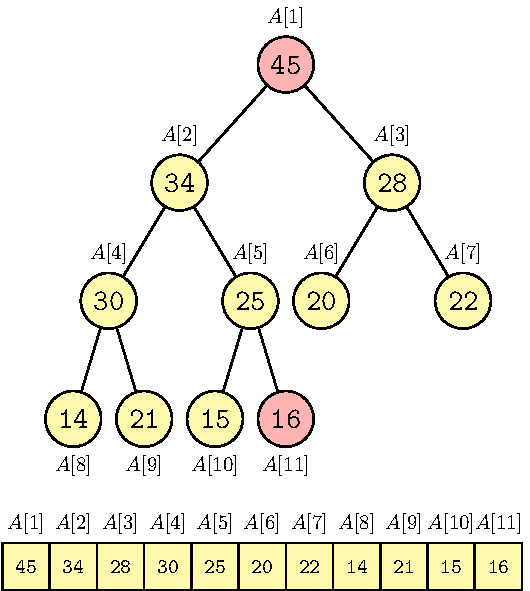
\includegraphics[width=\textwidth,page=1]{heapsort.pdf}
\onslide<2|handout:0>\includegraphics[width=\textwidth,page=2]{heapsort.pdf}
\onslide<3|handout:0>\includegraphics[width=\textwidth,page=3]{heapsort.pdf}
\onslide<4|handout:0>\includegraphics[width=\textwidth,page=4]{heapsort.pdf}
\onslide<5|handout:0>\includegraphics[width=\textwidth,page=5]{heapsort.pdf}
\onslide<6|handout:0>\includegraphics[width=\textwidth,page=6]{heapsort.pdf}
\onslide<7|handout:0>\includegraphics[width=\textwidth,page=7]{heapsort.pdf}
\onslide<8|handout:0>\includegraphics[width=\textwidth,page=8]{heapsort.pdf}
\onslide<9|handout:0>\includegraphics[width=\textwidth,page=9]{heapsort.pdf}
\onslide<10|handout:0>\includegraphics[width=\textwidth,page=10]{heapsort.pdf}
\onslide<11|handout:0>\includegraphics[width=\textwidth,page=11]{heapsort.pdf}
\onslide<12|handout:0>\includegraphics[width=\textwidth,page=12]{heapsort.pdf}
\onslide<13|handout:0>\includegraphics[width=\textwidth,page=13]{heapsort.pdf}
\onslide<14|handout:0>\includegraphics[width=\textwidth,page=14]{heapsort.pdf}
\onslide<15|handout:0>\includegraphics[width=\textwidth,page=15]{heapsort.pdf}
\onslide<16|handout:0>\includegraphics[width=\textwidth,page=16]{heapsort.pdf}
\onslide<17|handout:0>\includegraphics[width=\textwidth,page=17]{heapsort.pdf}
\onslide<18|handout:0>\includegraphics[width=\textwidth,page=18]{heapsort.pdf}
\onslide<19|handout:0>\includegraphics[width=\textwidth,page=19]{heapsort.pdf}
\onslide<20|handout:0>\includegraphics[width=\textwidth,page=20]{heapsort.pdf}
\onslide<21|handout:2>\includegraphics[width=\textwidth,page=21]{heapsort.pdf}
\end{overprint}
\column{0.46\textwidth}
\vspace{-9pt}
\begin{Procedure}
\caption[A]{\textsc{heapSort}($\Item[\,]\ A$, \INTEGER $n$)}
$\heapbuild(A, n)$\;
\For{$i = n$ \DOWNTO $2$}
{
  \alert<1,5,7,9,11,13,15,17,19>{$\Swap(A,1,i)$}\;
  \alert<2-4,6,8,10,12,14,16,18,20>{$\maxheapify(A, 1, i-1)$}\;
}
\end{Procedure}
\end{columns}
\end{frame}

\begin{frame}{Complessità}

\vspace{-9pt}
\begin{myboxtitle}[Complessità]
\BI
\item \heapbuild() costa $\Theta(n)$
\item \maxheapify() costa $\Theta(\log i)$ in un
heap con $i$ elementi
\item Viene eseguita con $i$ che varia da $2$ a $n$
\EI
\[
T(n) = \sum_{i=2}^n \log i + \Theta(n) = \Theta(n \log n)
\]
\end{myboxtitle}

\end{frame}

\begin{frame}{Correttezza}
    
\vspace{-9pt}
\begin{myboxtitle}[Invariante di ciclo]
\smallskip
Al passo $i$
\BIL
\item il sottovettore $A[i+1 \ldots n]$ è ordinato; 
\item $A[1 \ldots i] \leq A[i+1 \ldots n]$ 
\item $A[1]$ è la radice di un vettore heap di dimensione $i$.
\EIL
\end{myboxtitle}

\begin{myboxtitle}[Dimostrazione]
\smallskip
Per esercizio
\end{myboxtitle}

\end{frame}

\begin{frame}{Reality check}
\begin{myboxtitle}[Utilizzo (\url{https://en.wikipedia.org/wiki/Heapsort})]
\emph{Because of the $O(n \log n)$ upper bound on heapsort's running time and constant upper bound on its auxiliary storage, embedded systems with real-time constraints or systems concerned with security often use heapsort, such as the Linux kernel.}
\end{myboxtitle}

\end{frame}

\subsection{Implementazione code}

\begin{frame}{Implementazione code con priorità}

\vspace{-9pt}
\BB{Quale versione}
Implementiamo una min-priority queue, in quanto negli esempi che vedremo
in seguito daremo la precedenza a elementi con priorità minore

\BB{Dettagli implementativi}
\BIL
\item Vedremo come strutturare un vettore che memorizza coppie\\
  $\langle$ \textit{valore}, \textit{priorità} $\rangle$
\item Vedremo come implementare \minheapify()
\item Vedremo come implementare i singoli metodi
\EIL

\end{frame}

\begin{frame}{Memorizzazione}

\vspace{-9pt}
\begin{Procedure}
\caption[A]{\PriorityItem}

\INTEGER $\heapprio$\REMR{Priorità}
\Item $\heapitem$\REMR{Elemento}
\INTEGER $\heappos$\REMR{Posizione nel vettore heap}

\end{Procedure}

\begin{Procedure}
\caption[A]{\Swap($\PriorityItem[\,]$ $H$, \INTEGER $i$, \INTEGER $j$)}

$\PriorityItem\ \mathit{temp} = H[i]$\;
$H[i] = H[j]$\;
$H[j] = \mathit{temp}$\;
$H[i].\heappos = i$\;
$H[j].\heappos = j$\;

\end{Procedure}

\end{frame}

\begin{frame}{Inizializzazione}
    
\vspace{-9pt}
\begin{Procedure}
\caption[A]{\Heap}
$\INTEGER\ \heapsize$\REMR{Numero massimo di elementi nella coda}
$\INTEGER\ \heapcount$\REMR{Numero attuale di elementi nella coda}
$\PriorityItem[\,]\ H$\REMR{Vettore \emph{heap}}
\BlankLine

\PROCEDURE{\Heap \heapconstructor(\INTEGER\ $n$)}{
  $\Heap\ t = \NEW\ \Heap$\;
  $t.\heapsize = n$\;
  $t.\heapcount = 0$\;
  $t.H = \NEW\ \PriorityItem[1 \mldots n]$\;
  \Return $t$
}
\end{Procedure}

\end{frame}

\begin{frame}{Inserimento}

\vspace{-9pt}
\begin{Procedure}
\caption[A]{\PriorityItem\ \heapinsert(\Item $x$, \INTEGER\ $p$)}
\precondition{$\heapcount < \heapsize$}
\BlankLine
$\heapcount = \heapcount+1$\;
$H[\heapcount] = \NEW\ \PriorityItem()$\;
$H[\heapcount].\heapitem = x$\;
$H[\heapcount].\heapprio = p$\;
$H[\heapcount].\heappos = \heapcount$\;
\INTEGER $i = \heapcount$\;
\While{$i > 1$ \AND $H[i].\heapprio < H[\heapparent(i)].\heapprio$}
{
  $\Swap(H, i, \heapparent(i))$\;
  $i = \heapparent(i)$\;
}
\Return $H[i]$\;
\end{Procedure}


\end{frame}

\begin{frame}{minHeapRestore()}
    
\vspace{-9pt}
\begin{Procedure}
\caption[A]{\minheapify($\PriorityItem[\,]\ A$, \INTEGER $i$, \INTEGER \heapcount)}

\INTEGER $\Min = i$\;
\If{$\heapleft(i) \leq \heapcount$ \AND $A[\heapleft(i)].\heapprio < A[\Min].\heapprio$}
{
  $\Min = \heapleft(i)$
}
\If{$\heapright(i) \leq \heapcount$ \AND $A[\heapright(i)].\heapprio < A[\Min].\heapprio$}
{
  $\Min = \heapright(i)$
}
\If{$i \neq \Min$}
{
  $\Swap(A, i, \Min)$\;
  $\minheapify(A, \Min, \heapcount)$\;
}
\end{Procedure}

\end{frame}

\begin{frame}{Cancellazione / lettura minimo}

\vspace{-9pt}
\begin{Procedure}
\caption[A]{\Item\ \heapdeletemin()}
\precondition{$\heapcount > 0$}
\BlankLine
%$\Item \Temp = H[1]$\;
$\Swap(H, 1, \heapcount)$\;
$\heapcount = \heapcount-1$\;
$\minheapify(H, 1, \heapcount)$\;
\Return $H[\heapcount+1].\heapitem$\;
\end{Procedure}

\begin{Procedure}
\caption[A]{\Item \heapmin()}
  \PRECONDITION: $\heapcount > 0$\; 
  \BlankLine
  \Return $H[1].\heapitem$\;
\end{Procedure}

\end{frame}

\begin{frame}{Decremento priorità}

\vspace{-9pt}
\begin{Procedure}
\caption[A]{\heapdecrease(\PriorityItem\ $x$, \INTEGER\ $p$)}
\precondition{$p < x.\heapprio$}
\BlankLine
{
  $x.\heapprio = p$\;
  $\INTEGER\ i = x.\heappos$\;
  \While{$i > 1$ \AND $H[i].\heapprio < H[\heapparent(i)].\heapprio$}
  {
    $\Swap(H, i, \heapparent(i))$\;
    $i = \heapparent(i)$\; 
  }
}
\end{Procedure}


\end{frame}

\begin{frame}{Complessità}

\BB{
\BI
\item Tutte le operazioni che modificano gli heap sistemano la proprietà heap
\BI
\item lungo un cammino radice-foglia (\heapdeletemin()) 
\item oppure lungo un cammino nodo-radice (\heapinsert(), \heapdecrease())
\EI
\item Poichè l'altezza è $\lfloor \log n \rfloor$, il costo di tali operazioni è $O(\log n)$
\EI
}
\bigskip
\begin{tabular}{|l|l|}
\hline
\textbf{Operazione} & \textbf{Costo} \\\hline
\heapinsert() & $O(\log n)$ \\\hline
\heapdeletemin() & $O(\log n)$ \\\hline
\heapmin() & $\Theta(1)$ \\\hline
\heapdecrease() & $O(\log n)$ \\\hline
\end{tabular}
\end{frame}

\begin{frame}<1|handout:0>[noframenumbering]{Heap (mucchio) of presents}

\IG{0.8}{tree.png}

\end{frame}


\section{Insiemi disgiunti}

\subsection{Introduzione}

\begin{frame}{Insiemi disgiunti -- Merge-Find Set}

\vspace{-9pt}
\begin{myboxtitle}[Motivazioni]
\BIL
\item In alcune applicazioni siamo interessati a gestire una collezione 
$S = \{ S_1, S_2, \ldots, S_k \}$ di \alert{insiemi dinamici disgiunti}
  \smallskip
  \BI
  \item $\forall i,j: i \neq j \Rightarrow S_i \cap S_j = \emptyset$
  \item $\cup_{i=1}^k S_i = \cal S$, dove $n = |\cal S|$
  \EI
\item Esempio: componenti di un grafo
\EIL
\end{myboxtitle}

\begin{myboxtitle}[Operazioni fondamentali]
\BIL
\item Creare $n$ insiemi disgiunti, ognuno composto da un unico elemento
\item \fontproc{merge}(): Unire più insiemi
\item \fontproc{find}(): Identificare l'insieme a cui appartiene un elemento
\EIL
\end{myboxtitle}

\end{frame}


\begin{frame}{Insiemi disgiunti}

\vspace{-9pt}
\begin{myboxtitle}[Rappresentante]
\BIL
\item Ogni insieme è identificato da un \alert{rappresentante} univoco
\item Il rappresentante  dell'insieme $S_i$  è un qualunque membro di $S_i$
\item Operazioni di ricerca del rappresentante su uno stesso insieme devono restituire sempre lo stesso oggetto
\item Solo in caso di unione con altro insieme il rappresentante può cambiare
\EIL
\end{myboxtitle}

\begin{myboxtitle}[Memorizzazione]
Invece di memorizzare oggetti, utilizziamo gli interi $1 \ldots n$
e assumiamo che l'associazione intero-oggetto sia memorizzata esternamente
\end{myboxtitle}

\end{frame}

\begin{frame}{Specifica}

\vspace{-9pt}
\begin{Procedure}
\caption[A]{\mfset}

\BlankLine
\% Crea $n$ componenti $\{1\}, \mldots, \{n\}$\;
\mfset $\mfconstructor(\INTEGER\ n)$\;

\BlankLine
\% Restituisce il rappresentante della componente contenente $x$\;
\INTEGER\ $\mffind(\INTEGER\ x)$\;

\BlankLine
\% Unisce le componenti che contengono $x$ e $y$\;
$\mfmerge(\INTEGER\ x, \INTEGER\ y)$\;
 
\BlankLine
\end{Procedure}

\end{frame}

\begin{frame}{Esempio}
\vspace{-9pt}
\IG{1.0}{mfset-esempio.pdf}
\end{frame}

\begin{frame}{Applicazione: Componenti connesse dinamiche}

\vspace{-9pt}
\begin{myboxtitle}[Problema]
Trovare le componenti connesse di un grafo non orientato \alert{dinamico}
\end{myboxtitle}

\begin{columns}[T]
\column{0.53\textwidth}
\vspace{-9pt}
\begin{myboxtitle}[Algoritmo]
\BIL
\item Si inizia con componenti connesse costituite da un unico vertice
\item Per ogni $(u,v) \in E$, si esegue $\fontproc{merge}(u, v)$ 
\item Ogni insieme disgiunto rappresenta
una componente connessa
\EIL
\end{myboxtitle}
\column{0.45\textwidth}
\vspace{-9pt}
\begin{Procedure}
\caption[A]{\mfset\ \connectedcomponents($\Graph\ G$)}

\mfset $M = \mfconstructor(G.n)$\;
\ForEach{$u \in G.V()$}
{
  \ForEach{$v \in G.\adj(u)$}
  {
    $M.\mfmerge(u, v)$\;
  }
}
\Return\ $M$\;
\end{Procedure}

\end{columns}

\end{frame}

\begin{frame}{Applicazione: Componenti connesse dinamiche}

\vspace{-9pt}
\begin{myboxtitle}[Complessità]
\smallskip
$O(n) + m$ operazioni $\fontproc{merge}()$
\end{myboxtitle}

\begin{myboxtitle}[Motivazione]
\smallskip
Questo algoritmo è interessante per la capacità di gestire grafi dinamici 
(in cui gli archi vengono aggiunti)
\end{myboxtitle}

\end{frame}

\subsection{Realizzazione basata su liste}


\begin{frame}{Realizzazione basata su insiemi di liste}

\vspace{-9pt}
\BB{Ogni insieme viene rappresentato da una lista concatenata}
\BIL
\item Il primo oggetto di una lista è il rappresentante dell'insieme
\item Ogni elemento nella lista contiene:
  \BI
  \item un oggetto
  \item un puntatore all'elemento successivo
  \item un puntatore al rappresentante
  \EI
\EIL

\IG{1.0}{mfset-liste.pdf}

\end{frame}

\begin{frame}{Operazione $\fontproc{find}(x)$}

\vspace{-9pt}
\BIL
\item Si restituisce il rappresentante di $x$
\item L'operazione $\fontproc{find}(x)$ richiede tempo $O(1)$
\EIL

\bigskip
\IG{1.0}{mfset-liste.pdf}

\end{frame}


\begin{frame}{Operazione $\fontproc{merge}(x,y)$}

\vspace{-9pt}
\BIL
\item Si "appende" la lista che contiene $y$ alla lista che contiene $x$, modificando
i puntatori ai rappresentanti nella lista "appesa"
\item Costo nel caso pessimo per $n$ operazioni: $O(n^2)$
\item Costo ammortizzato: $O(n)$
\EIL

\IG{0.7}{mfset-liste-merge.pdf}

\end{frame}

\subsection{Realizzazione basata su alberi}

\begin{frame}{Realizzazione basata su insieme di alberi (foresta)}

\vspace{-9pt}
\BB{Ogni insieme viene rappresentato da un albero}

\begin{columns}[T]
\column{0.65\textwidth}
\BIL
\item Ogni nodo dell'albero contiene:
  \BI
  \item un oggetto
  \item un puntatore al padre
  \EI
\item La radice è il rappresentante dell'insieme
\item La radice ha un puntatore a se stessa
\EIL
\column{0.30\textwidth}
\IG{1.0}{mfset-alberi.pdf}
\end{columns}

\end{frame}



\begin{frame}{Operazione $\fontproc{merge}(x,y)$}

\vspace{-9pt}
\BIL
\item Si aggancia l'albero radicato in $y$ ad $x$
\item Modificando il puntatore al padre di $y$
\item Costo: $O(1)$
\EIL

\bigskip\centering
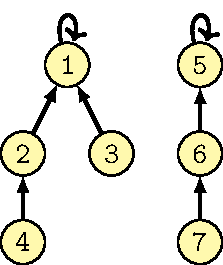
\includegraphics[width=0.23\textwidth,page=1,valign=t]{mfset-alberi.pdf}
\qquad{\huge $\Rightarrow$}\quad
\includegraphics[width=0.23\textwidth,page=2,valign=t]{mfset-alberi.pdf}




\end{frame}

\begin{frame}{Operazione $\fontproc{find}(x)$}

\vspace{-9pt}
\begin{columns}[T]
\column{0.65\textwidth}
\BIL
\item Risale la lista dei padri di $x$ fino a trovare la radice e 
restituisce la radice come rappresentante
\item Costo: $O(n)$ nel caso pessimo (perché?)
\EIL
\column{0.30\textwidth}
\vspace{-9pt}
\IG{1.0}{mfset-alberi.pdf}
\end{columns}

\end{frame}

\subsection{Euristiche}

\begin{frame}{Tecniche euristiche}

\vspace{-9pt}
\begin{myboxtitle}[Algoritmo euristico]
\EE un particolare tipo di algoritmo progettato per 
\BI
\item risolvere un problema  più velocemente, qualora i metodi classici 
siano troppo lenti
\item trovare una soluzione approssimata, qualora i metodi classici 
falliscano nel trovare una soluzione esatta
\EI
\end{myboxtitle}

\begin{myboxtitle}[Euristiche applicate agli insiemi disgiunti]
\BIL
\item Euristica del \alert{peso} (Liste)
\item Euristica del \alert{rango} (Alberi)
\item Euristica della \alert{compressione dei cammini} (Alberi)
\EIL
\end{myboxtitle}

\end{frame}

\begin{frame}{Liste: Euristica sul peso}

\vspace{-9pt}
\begin{myboxtitle}[Strategia per diminuire il costo dell'operazione \fontproc{merge}()]
\BIL
\item Memorizzare nelle liste l’informazione sulla loro lunghezza
\item Agganciare la lista più corta a quella più lunga
\item La lunghezza della lista può essere mantenuta in tempo $O(1)$
\EIL 
\end{myboxtitle}

\begin{myboxtitle}[Complessità]
\BIL
\item \EE possibile dimostrare che il costo delle operazioni $\fontproc{find}()$ è limitato superiormente da $O(\log n)$.
\EIL
\end{myboxtitle}
\end{frame}

\begin{frame}{Alberi: Euristica sul rango}

\vspace{-9pt}
\begin{myboxtitle}[Strategia per diminuire il costo dell'operazione \fontproc{find}()]
\BIL
\item Ogni nodo mantiene informazioni sul proprio rango
\item Il rango $\mathit{rank}[x]$ di un nodo $x$ è il numero di archi 
del cammino più lungo fra $x$ e una foglia sua discendente
\item Rango $\equiv$ altezza del sottoalbero associato al nodo
\item Obiettivo: mantenere bassa l'altezza degli alberi
\EIL 
\end{myboxtitle}

\end{frame}

\begin{frame}{Alberi: Euristica sul rango}

\vspace{-15pt}
\TwoCols{
\BB{Alberi di rango uguale}
\BIL
\item Si aggancia un albero alla radice
dell'altro (indifferente)
\item L'altezza cresce di 1
\EIL
\bigskip
\includegraphics<1|handout:0>[width=0.37\textwidth,page=1,valign=t]{mfset-alberi.pdf}
\quad{\huge $\Rightarrow$}
\includegraphics<1|handout:0>[width=0.37\textwidth,page=2,valign=t]{mfset-alberi.pdf}
}{
\BB{Alberi di rango diverso}
\BIL
\item Si aggancia l'albero con rango più basso all'albero con rango più alto
\item L'altezza resta inalterata
\EIL
\bigskip
\includegraphics<1|handout:0>[width=0.37\textwidth,page=3,valign=t]{mfset-alberi.pdf}
\quad{\huge $\Rightarrow$}
\includegraphics<1|handout:0>[width=0.37\textwidth,page=4,valign=t]{mfset-alberi.pdf}

}

\end{frame}

\begin{frame}{Complessità}

\vspace{-9pt}
\begin{myboxtitle}[Teorema]
Un albero \mfset con radice $r$ ottenuto tramite euristica sul rango ha almeno
$2^{\mfrank[r]}$ nodi.
\end{myboxtitle}

\begin{myboxtitle}[Dimostrazione (informale)]
\begin{overprint}
\onslide<1|handout:1>
\BIL
\item \textbf{Induzione caso base}: All'inizio tutti gli alberi sono costituiti da un nodo singolo, con rank 0;
\item quindi ogni albero ha almeno $2^0=1$ nodi, corretto.
\EIL
\onslide<2|handout:2>
\BIL
\item \textbf{Induzione caso 1}:
Facendo merge di due alberi con radici\\ $x$, $y$ con rango 
$\mathit{rank}[x] > \mathit{rank}[y]$

\smallskip
\BIL
\item il rango finale è pari a $\mathit{rank}[x]$
\item Per induzione, il numero di nodi è ${} \geq 2^{\mathit{rank}[x]} + 2^{\mathit{rank}[y]}$, 
che è maggiore di $2^{\mathit{rank}[x]}$.
\EIL
\EIL
\onslide<3|handout:3>
\BIL
\item \textbf{Induzione caso 2}: Facendo merge di due alberi con radici\\ $x$, $y$ con rango $\mathit{rank}[x] = \mathit{rank}[y]$, 

\smallskip
\BIL
\item il rango finale è pari a $\mathit{rank}[x]+1$ 
\item Per induzione, il numero di nodi è $\geq$ 
\[
  2^{\mathit{rank}[x]}+2^{\mathit{rank}[y]} = 2^{\mathit{rank}[x]} + 2^{\mathit{rank}[x]} = 2^{\mathit{rank}[x]+1}
\]
\EIL
come volevasi dimostrare

\EIL
\end{overprint}
\end{myboxtitle}



\end{frame}

\begin{frame}{Complessità}


\vspace{-9pt}
\begin{myboxtitle}[Corollario]
Un albero \mfset con radice $r$ ed $n$ nodi ha altezza inferiore a $\log n$.

\end{myboxtitle}

\begin{myboxtitle}[Dimostrazione]
\[
  n \geq 2^{\mfrank[r]} \Leftrightarrow \mfrank[r] \leq \log n
\]
\end{myboxtitle}

\begin{myboxtitle}[Complessità]
L'operazione $\fontproc{find}(x)$ ha costo $O(\log n)$
\end{myboxtitle}


\end{frame}

\begin{frame}{Algoritmo}

\vspace{-15pt}
\begin{columns}[T]
\column{0.43\textwidth}
\begin{Procedure}
\caption[T]{\mfset \phantom{\mfmerge($\INTEGER\ x, \INTEGER\ y$)}}	

$\INTEGER[\,]\ \mfparent$\;
$\INTEGER[\,]\ \mfrank$\;
\BlankLine

\mfset \PROCEDURE{\mfconstructor(\INTEGER $n$)}
{
  $\mfset\ t = \NEW\ \mfset$\;
  $t.\mfparent = \INTEGER[1 \mldots n]$\;
  $t.\mfrank = \INTEGER[1 \mldots n]$\;
  \For{$i = 1$ \TO\ $n$}
  {
    $t.\mfparent[i] = i$\;
    $t.\mfrank[i] = 0$\;
  }
  \Return $t$\;
}
\end{Procedure}

\column{0.55\textwidth}
\begin{Procedure}
\caption[A]{\mfmerge($\INTEGER\ x, \INTEGER\ y$)}
{
  $r_x = \mffind(x)$\;
  $r_y = \mffind(y)$\;
  \If{$r_x \neq r_y$}
  {
    \uIf{$\mfrank[r_x] > \mfrank[r_y]$}
    {
      $\mfparent[r_y] = r_x$\;
    }
    \uElseIf{$\mfrank[r_y] > \mfrank[r_x]$}
    {
      $\mfparent[r_x] = r_y$\;
    }
    \Else
    {
      $\mfparent[r_x] = r_y$\;
      $\mfrank[r_y] = \mfrank[r_y]+1$
    }
  }
}
\end{Procedure}
\end{columns}

\end{frame}

\begin{frame}{Alberi: Euristica di compressione dei cammini}

\vspace{-15pt}
\begin{columns}[T]
\column{0.48\textwidth}
\begin{myboxtitle}[Operazione $\fontproc{find}(x)$]
L'albero viene "appiattito" in modo che 
ricerche successive di $x$ siano svolte in $O(1)$
\end{myboxtitle}

\smallskip\centering
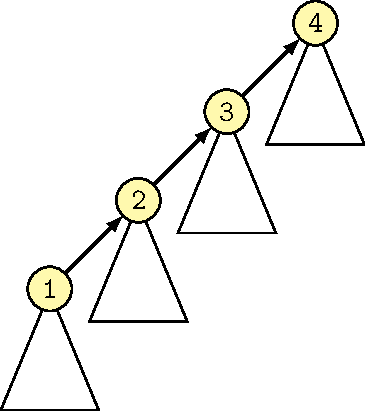
\includegraphics[width=0.7\textwidth,page=1]{mfset-compressione.pdf}
\column{0.48\textwidth}
\begin{Procedure}
\caption[A]{\INTEGER\ \mffind($\INTEGER\ x$)}
  \If{$\mfparent[x] \neq x$}{$\mfparent[x] = \mffind(\mfparent[x])$}
  \Return $\mfparent[x]$\;
\end{Procedure}
\includegraphics[width=1\textwidth,page=2]{mfset-compressione.pdf}
\end{columns}
\end{frame}


\begin{frame}{Alberi: Euristica sul rango + compressione cammini}

\vspace{-9pt}
\begin{myboxtitle}[Applicando entrambe le euristiche]
\BIL
\item Il rango non è più l'altezza del nodo, ma il \alert{limite superiore} all'altezza del nodo
\item \alert{Non} viene calcolato il rango corretto
\BI
\item Troppo difficile mantenere le informazioni di rango corretto
\item In ogni caso, non è necessario
\EI
\EIL
\end{myboxtitle}

\begin{myboxtitle}[Complessità]
\BIL 
\item Costo ammortizzato di $m$ operazioni merge-find in un insieme di $n$
elementi è $O(m \cdot \alpha(n))$
\item  La \alert{funzione inversa di Ackermann $\alpha(n)$} crescente lentamente
\item Esempi: per $n \leq 2^{65536}$, $\alpha(n) \leq 5$
\EIL
\end{myboxtitle}

\end{frame}

\begin{frame}{Complessità -- Riassunto}

\begin{tabular}{|P{6cm}|l|l|}
\hline
\textbf{Algoritmo} & \fontproc{find}() & \fontproc{merge}() \\\hline
Liste  & $O(1)$ & $O(n)$ \\\hline
Alberi & $O(n)$ & $O(1)^+$ \\\hline
Liste + Euristica sul peso & $O(1)$ & $O(\log n)^*$ \\\hline
Alberi + Euristica sul rango & $O(\log n)$ & $O(1)^+$ \\\hline
Alberi + Euristica sul rango +
Compressione cammini & $O(1)^*$ & $O(1)$ \\\hline
\end{tabular}

\bigskip
$^*$ Complessità ammortizzata\\
$^+$ Si considera solo l'operazione di unione, non si considera l'identificazione dei rappresentanti tramite \fontproc{find}()

\bigskip
Se interessati all'analisi ammortizzata per alberi + euristica sul rango + compressione cammini, consultate questi appunti:\\

\medskip
\footnotesize
\url{http://jeffe.cs.illinois.edu/teaching/algorithms/notes/11-unionfind.pdf}


\end{frame}

\end{document}
